\section{RMSE plots for other settings}
\label{sec:other-settings}

Here we plot the RMSE improvements through amplification and optimization for number of epochs in $\{8, 16, 32\}$ and iterations per epoch in $\{32, 64, 128\}$.

\subsection{Number of epochs $=8$ and iterations per epoch $=32$}
\begin{figure}[H]
    \centering
    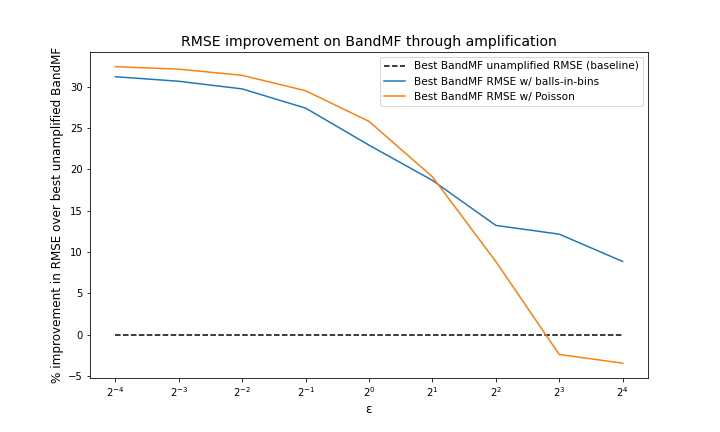
\includegraphics[width=0.8\linewidth]{rmse-plots/32_8_RMSE-improvement-on-BandMF-through-amplification.png}
    \caption{Improvement in RMSE over unamplified $b$-banded matrix factorization due to different amplification schemes. All curves optimize the choice of $b$ at each point.}
\end{figure}

\begin{figure}[H]
    \centering
    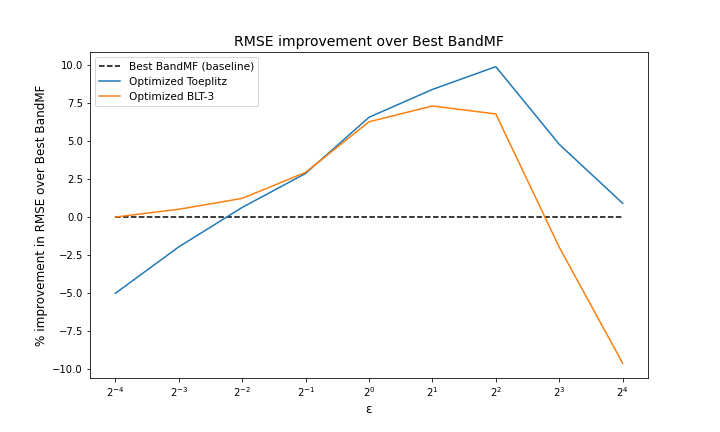
\includegraphics[width=.8\linewidth]{rmse-plots/32_8_RMSE-improvement-over-Best-BandMF.png}
    \caption{Improvement from optimizing $\bfC$ using objective accounting for amplification.}
\end{figure}

\subsection{Number of epochs $=8$ and iterations per epoch $=64$}
\begin{figure}[H]
    \centering
    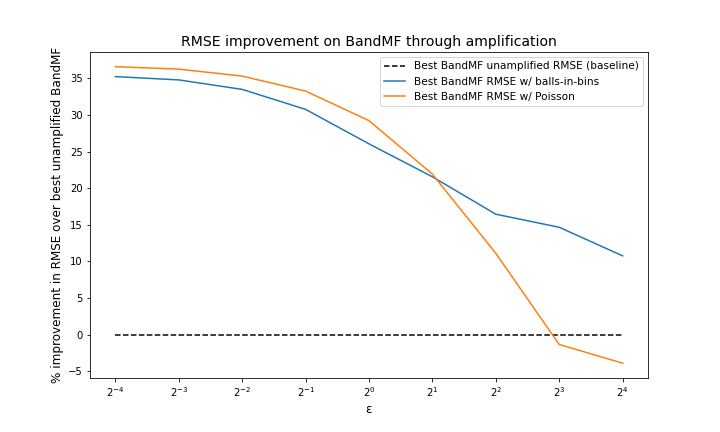
\includegraphics[width=0.8\linewidth]{rmse-plots/64_8_RMSE-improvement-on-BandMF-through-amplification.png}
    \caption{Improvement in RMSE over unamplified $b$-banded matrix factorization due to different amplification schemes. All curves optimize the choice of $b$ at each point.}
\end{figure}

\begin{figure}[H]
    \centering
    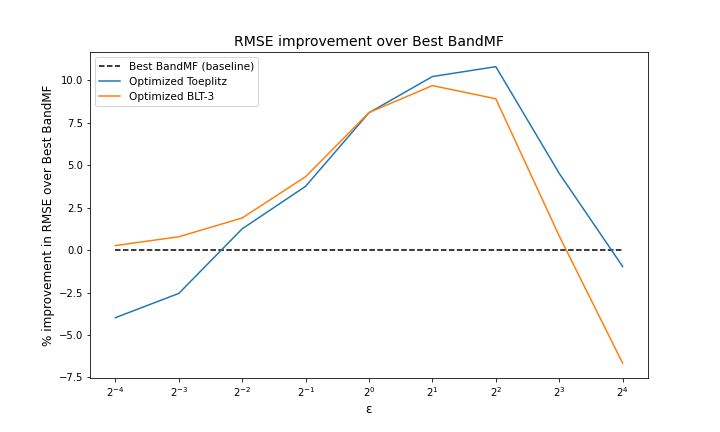
\includegraphics[width=.8\linewidth]{rmse-plots/64_8_RMSE-improvement-over-Best-BandMF.png}
    \caption{Improvement from optimizing $\bfC$ using objective accounting for amplification.}
\end{figure}

\subsection{Number of epochs $=8$ and iterations per epoch $=128$}
\begin{figure}[H]
    \centering
    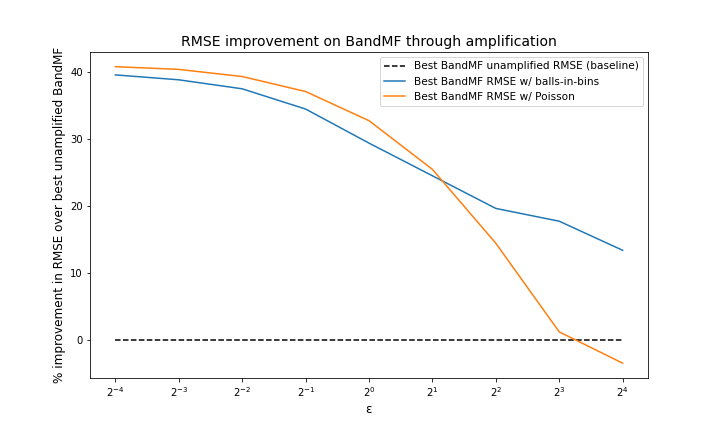
\includegraphics[width=0.8\linewidth]{rmse-plots/128_8_RMSE-improvement-on-BandMF-through-amplification.png}
    \caption{Improvement in RMSE over unamplified $b$-banded matrix factorization due to different amplification schemes. All curves optimize the choice of $b$ at each point.}
\end{figure}

\begin{figure}[H]
    \centering
    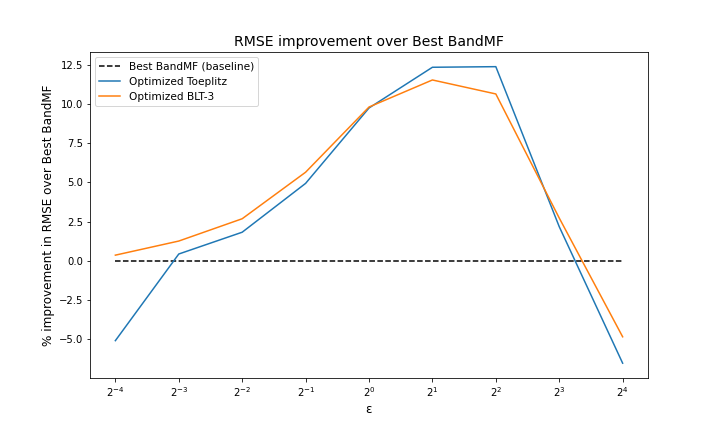
\includegraphics[width=.8\linewidth]{rmse-plots/128_8_RMSE-improvement-over-Best-BandMF.png}
    \caption{Improvement from optimizing $\bfC$ using objective accounting for amplification.}
\end{figure}

\subsection{Number of epochs $=16$ and iterations per epoch $=32$}
\begin{figure}[H]
    \centering
    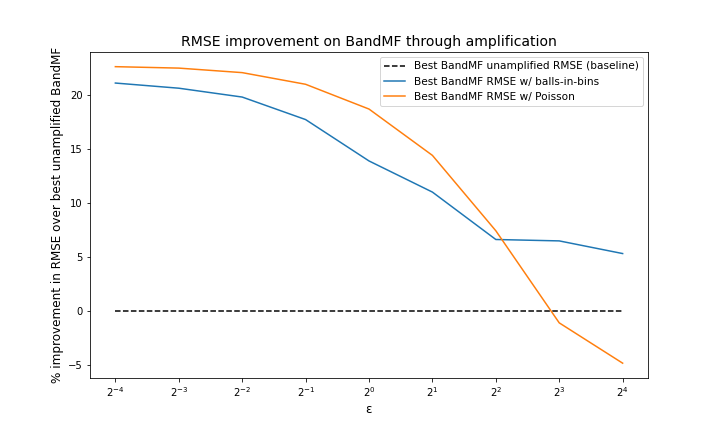
\includegraphics[width=0.8\linewidth]{rmse-plots/32_16_RMSE-improvement-on-BandMF-through-amplification.png}
    \caption{Improvement in RMSE over unamplified $b$-banded matrix factorization due to different amplification schemes. All curves optimize the choice of $b$ at each point.}
\end{figure}

\begin{figure}[H]
    \centering
    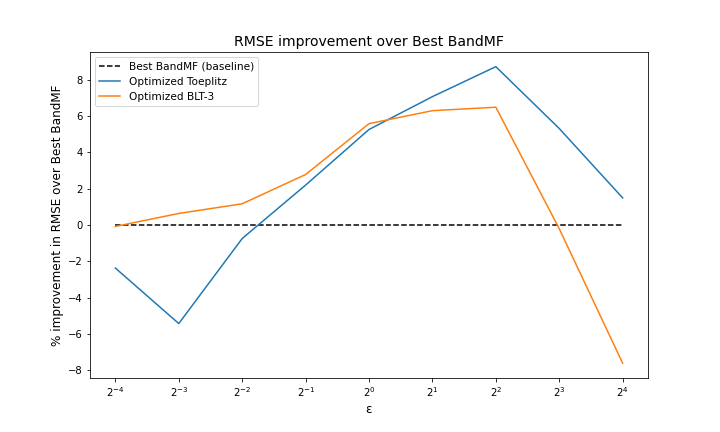
\includegraphics[width=.8\linewidth]{rmse-plots/32_16_RMSE-improvement-over-Best-BandMF.png}
    \caption{Improvement from optimizing $\bfC$ using objective accounting for amplification.}
\end{figure}

\subsection{Number of epochs $=16$ and iterations per epoch $=64$}
\begin{figure}[H]
    \centering
    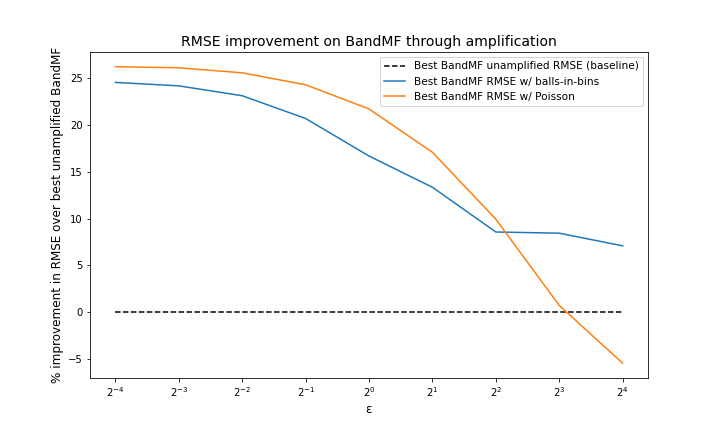
\includegraphics[width=0.8\linewidth]{rmse-plots/64_16_RMSE-improvement-on-BandMF-through-amplification.png}
    \caption{Improvement in RMSE over unamplified $b$-banded matrix factorization due to different amplification schemes. All curves optimize the choice of $b$ at each point.}
\end{figure}

\begin{figure}[H]
    \centering
    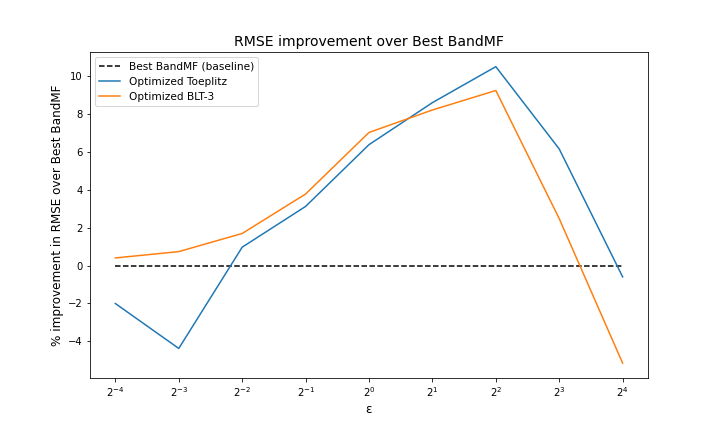
\includegraphics[width=.8\linewidth]{rmse-plots/64_16_RMSE-improvement-over-Best-BandMF.png}
    \caption{Improvement from optimizing $\bfC$ using objective accounting for amplification.}
\end{figure}

\subsection{Number of epochs $=16$ and iterations per epoch $=128$}
\begin{figure}[H]
    \centering
    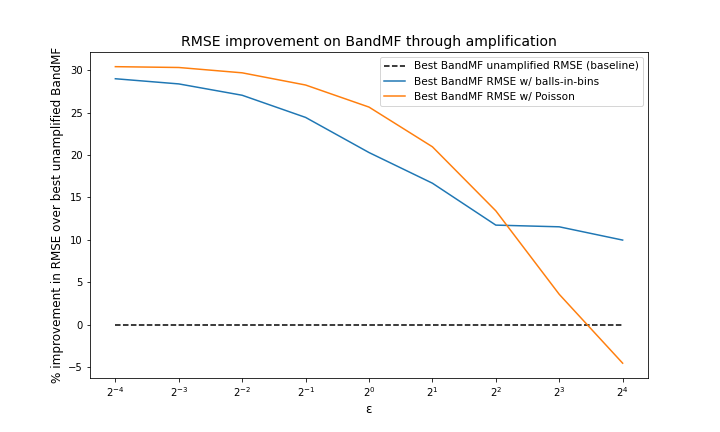
\includegraphics[width=0.8\linewidth]{rmse-plots/128_16_RMSE-improvement-on-BandMF-through-amplification.png}
    \caption{Improvement in RMSE over unamplified $b$-banded matrix factorization due to different amplification schemes. All curves optimize the choice of $b$ at each point.}
\end{figure}

\begin{figure}[H]
    \centering
    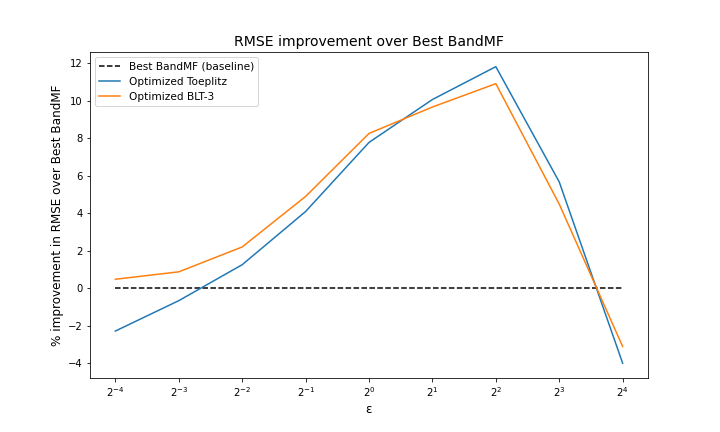
\includegraphics[width=.8\linewidth]{rmse-plots/128_16_RMSE-improvement-over-Best-BandMF.png}
    \caption{Improvement from optimizing $\bfC$ using objective accounting for amplification.}
\end{figure}


\subsection{Number of epochs $=32$ and iterations per epoch $=32$}
\begin{figure}[H]
    \centering
    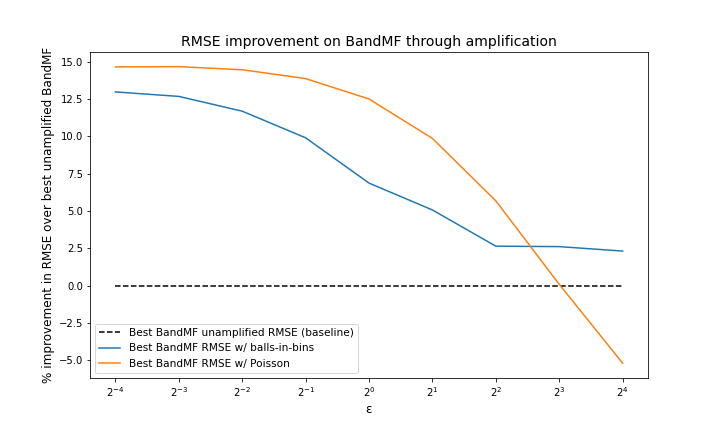
\includegraphics[width=0.8\linewidth]{rmse-plots/32_32_RMSE-improvement-on-BandMF-through-amplification.png}
    \caption{Improvement in RMSE over unamplified $b$-banded matrix factorization due to different amplification schemes. All curves optimize the choice of $b$ at each point.}
\end{figure}

\begin{figure}[H]
    \centering
    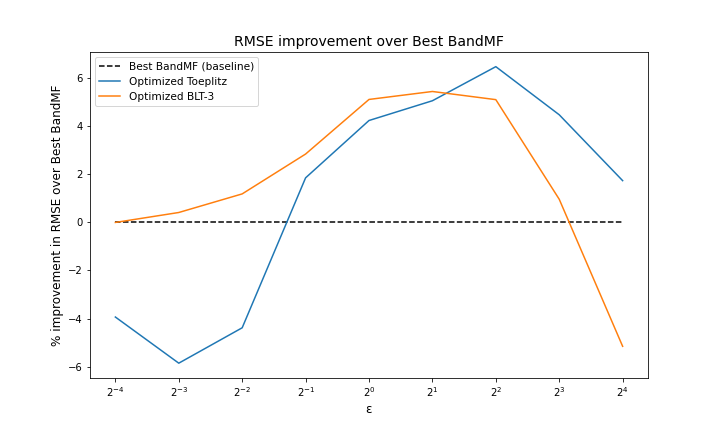
\includegraphics[width=.8\linewidth]{rmse-plots/32_32_RMSE-improvement-over-Best-BandMF.png}
    \caption{Improvement from optimizing $\bfC$ using objective accounting for amplification.}
\end{figure}

\subsection{Number of epochs $=32$ and iterations per epoch $=64$}
\begin{figure}[H]
    \centering
    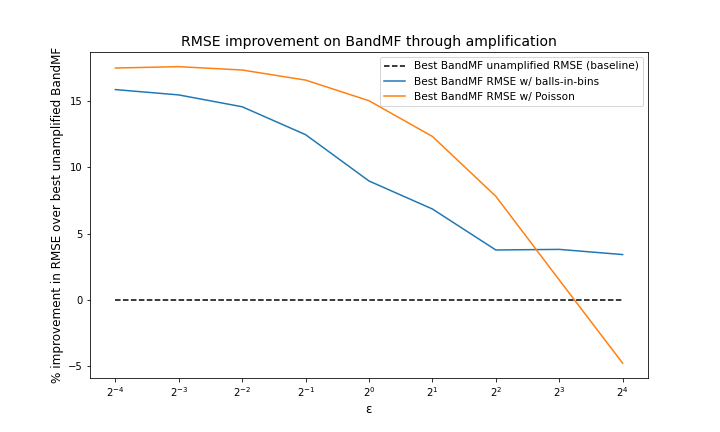
\includegraphics[width=0.8\linewidth]{rmse-plots/64_32_RMSE-improvement-on-BandMF-through-amplification.png}
    \caption{Improvement in RMSE over unamplified $b$-banded matrix factorization due to different amplification schemes. All curves optimize the choice of $b$ at each point.}
\end{figure}

\begin{figure}[H]
    \centering
    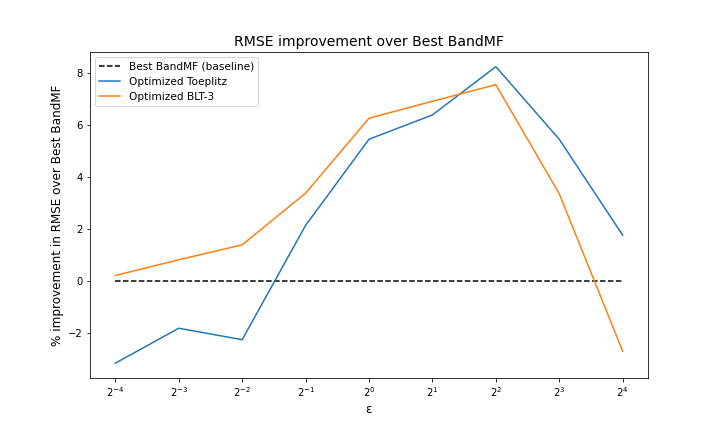
\includegraphics[width=.8\linewidth]{rmse-plots/64_32_RMSE-improvement-over-Best-BandMF.png}
    \caption{Improvement from optimizing $\bfC$ using objective accounting for amplification.}
\end{figure}

\subsection{Number of epochs $=32$ and iterations per epoch $=128$}
\begin{figure}[H]
    \centering
    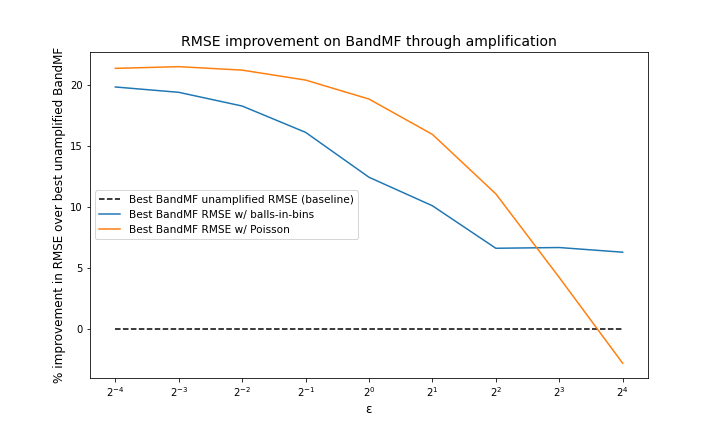
\includegraphics[width=0.8\linewidth]{rmse-plots/128_32_RMSE-improvement-on-BandMF-through-amplification.png}
    \caption{Improvement in RMSE over unamplified $b$-banded matrix factorization due to different amplification schemes. All curves optimize the choice of $b$ at each point.}
\end{figure}

\begin{figure}[H]
    \centering
    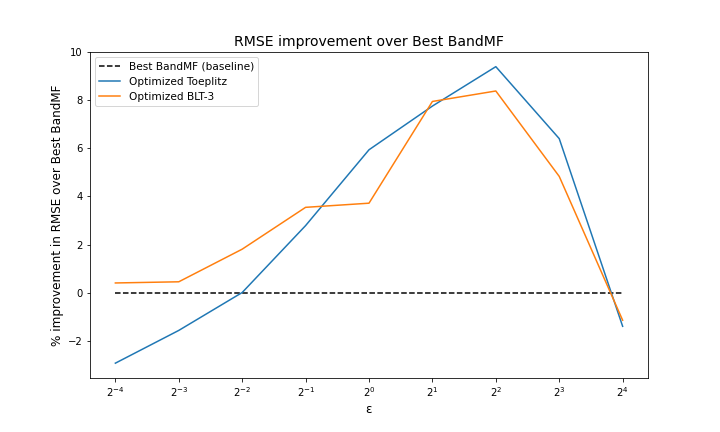
\includegraphics[width=.8\linewidth]{rmse-plots/128_32_RMSE-improvement-over-Best-BandMF.png}
    \caption{Improvement from optimizing $\bfC$ using objective accounting for amplification.}
\end{figure}